\documentclass[12pt]{article}

\usepackage[english]{babel}
\usepackage[utf8]{inputenc}
\usepackage{mathtools}
\usepackage{amssymb}
\usepackage{amsmath}
\usepackage{amsthm}
\usepackage{enumerate}
\usepackage{enumitem}
\usepackage{tikz-cd}
\usepackage{subcaption}
\usepackage[left=2cm,top=2.5cm,right=1.5cm,bottom=2.5cm]{geometry}
\setlength{\parindent}{0pt}

\newtheorem*{theorem}{Theorem}
\newtheorem*{proposition}{Proposition}
\theoremstyle{definition}
\newtheorem*{definition}{Definition}
\newtheorem*{remark}{Remark}
\newtheorem*{example}{Example}

\DeclareMathOperator{\Hom}{Hom}
\DeclareMathOperator{\Spec}{Spec}

\title{\Huge{Seminar in Toric Varieties}\\\vspace{5mm}\Large{Talk 3: Affine Toric Varieties}}
\author{Alejandro Plaza Gall\'{a}n}
\date{30 May 2022}

\begin{document}
\maketitle

\section{Group ring of a monoid}
\begin{definition}
A \textbf{monoid} $(S,+)$ is a set $S$ together with an associative operation $+:S\times S\rightarrow S$ that has a neutral element $0\in S$.

If the operation $+$ is commutative, then $S$ is called a commutative monoid.

A monoid homomorphism $x:S_1\rightarrow S_2$ between two monoids $(S_1,+_1),(S_2,+_2)$ is a map such that:
\begin{itemize}
\item for all $u,u'\in S_1$, $x(u+_1u')=x(u)+_2x(u')$,
\item $x(0_1)=0_2$.
\end{itemize}
\end{definition}

\begin{example}
$(\mathbb{N}_0,+)$, $(\mathbb{Z},+)$, $(\mathbb{C},\,\cdot\,)$.
\end{example}

\begin{definition}
Let $S$ be a commutative monoid. Let $\{u_i\}_{i\in I}\subseteq S$ be a family of elements in $S$.

We say that $\{u_i\}_{i\in I}$ are generators of $S$ if
\[S=\sum_{i\in I}\mathbb{N}_0u_i,\]
i.e. if $\forall s\in S$ $\exists u_{i_1},\ldots,u_{i_n}$, $\exists\lambda_1,\ldots,\lambda_n\in\mathbb{N}_0$ such that $s=\lambda_1u_{i_1}+\cdots+\lambda_nu_{i_n}$.

In case there is a finite family of generators, we say that $S$ is finitely generated.
\end{definition}

\begin{example}
$\mathbb{N}_0^n$ is a monoid with generators $e_1,\ldots,e_n$.

Every $(\lambda_1,\ldots,\lambda_n)\in\mathbb{N}_0^n$ can be expressed as
\[(\lambda_1,\ldots,\lambda_n)=\lambda_1e_1+\cdots+\lambda_ne_n.\]

$\mathbb{Z}^n$ is a monoid with generators $e_1,-e_1,\ldots,e_n,-e_n$.

Every $(\lambda_1,\ldots,\lambda_n)\in\mathbb{Z}^n$ can be expressed as
\[(\lambda_1,\ldots,\lambda_n)=\lambda_1^+e_1+\lambda_1^-(-e_1)+\cdots+\lambda_n^+e_n+\lambda_n^-(-e_n),\]
where
\[\lambda_i^+=\left\{\begin{array}{lll}\lambda_i&\text{if}&\lambda_i\geq0,\\0&\text{if}&\lambda_i<0,\end{array}\right.\hspace{5mm}\lambda_i^-=\left\{\begin{array}{lll}0&\text{if}&\lambda_i\geq0,\\-\lambda_i&\text{if}&\lambda_i<0.\end{array}\right.\]
\end{example}

\begin{definition}
Given a commutative monoid $S$, we define its \textbf{group ring} $\mathbb{C}[S]$ to be
\[\mathbb{C}[S]\coloneqq\bigoplus_{u\in S}\mathbb{C}\chi^u,\]
with the multiplication
\begin{align*}
\cdot:\mathbb{C}[S]\times\mathbb{C}[S]&\longrightarrow\mathbb{C}[S].\\
(\chi^u,\chi^{u'})&\longmapsto\chi^{u+u'}
\end{align*}
\end{definition}

Note that $\bigoplus_{u\in S}\mathbb{C}\chi^u$ is defined as the $\mathbb{C}$-vector space that has $S$ as a basis.

\begin{proposition}
\begin{enumerate}[label=\arabic*)]
\item The group ring is in fact a commutative $\mathbb{C}$-algebra with unit $\chi^0$.

\item If $\{u_i\}_{i\in I}$ is a system of generators of $S$, then $\{\chi^{u_i}\}_{i\in I}$ is a system of generators of $\mathbb{C}[S]$ as a $\mathbb{C}$-algebra.

\item In particular, if $S$ is finitely generated, then $\mathbb{C}[S]$ is a $\mathbb{C}$-affine algebra, i.e. it is finitely generated.
\end{enumerate}
\end{proposition}

\begin{proof}
\begin{enumerate}[label=\arabic*)]
\item By definition, $\mathbb{C}[S]$ is a $\mathbb{C}$-vector space. If we want the multiplication to satisfy associativity and distributivity, it must be defined as
\[\left(\sum_{i=1}^n\lambda_i\chi^{u_i}\right)\left(\sum_{j=1}^m\mu_j\chi^{u_j}\right)=\sum_{i=1}^m\sum_{j=1}^n\lambda_i\mu_j\chi^{u_i+u_j}.\]

Check: $\chi^0$ is the unity, the distributivity, the compatibility with scalars, the associativity and the commutativity.

\item Let $\sum_{j=1}^m\mu_j\chi^{v_j}\in\mathbb{C}[S]$. We can choose generators $u_1,\ldots,u_n$ such that
\[v_j=\sum_{i=1}^n\lambda_{ij}u_i,\]
for some $\lambda_{ij}\in\mathbb{N}_0$.
Hence,
\[\sum_{j=1}^m\mu_j\chi^{v_j}=\sum_{j=1}^m\mu_j\chi^{\sum_{i=1}^n\lambda_{ij}u_i}=\sum_{j=1}^m\mu_j(\chi^{u_1})^{\lambda_{1j}}\cdots(\chi^{u_n})^{\lambda_{nj}}.\]
Thus, $\{\chi^{u_i}\}_{i\in I}$ generate $\mathbb{C}[S]$ as a $\mathbb{C}$-algebra.
\end{enumerate}
\end{proof}

\begin{proposition}
Given a homomorphism $x:S_1\rightarrow S_2$ of commutative monoids, there exists a unique $\mathbb{C}$-algebra homomorphism $\varphi:\mathbb{C}[S_1]\rightarrow\mathbb{C}[S_2]$ such that $\forall u\in S_1$ $\varphi(\chi^u)=\chi^{x(u)}$.
\begin{itemize}
\item $x$ is injective if and only if $\varphi$ injective.

\item $x$ is surjective if and only if $\varphi$ is surjective.

\item In particular, if $x$ is a monoid isomorphism, then $\varphi$ is a $\mathbb{C}$-algebra isomorphism.
\end{itemize}
\end{proposition}

\begin{proof}
Let $x:S_1\rightarrow S_2$ be a monoid homomorphism. Define
\begin{align*}
\varphi:\mathbb{C}[S_1]&\longrightarrow\mathbb{C}[S_2].\\
\sum_{i=1}^n\lambda_i\chi^{u_i}&\longmapsto\sum_{i=1}^n\lambda_i\chi^{x(u_i)}
\end{align*}

We already know from linear algebra that a map $x:S_1\rightarrow S_2$ between bases of two vector spaces defines a unique linear map $\varphi$ between the vector spaces. The only thing remaining to show is that our $\varphi$ preserves the multiplication.

Check: $\varphi$ preserves the multiplication.

The points about injectivity and surjectivity of $x$ and $\varphi$ follow from the already known structure of vector spaces.
\end{proof}

\begin{proposition}
\begin{enumerate}[label=\arabic*)]
\item $\mathbb{C}[\mathbb{N}_0^n]\cong\mathbb{C}[X_1,\ldots,X_n]$.

\item $\mathbb{C}[\mathbb{Z}^n]\cong\mathbb{C}[X_1,X_1^{-1},\ldots,X_n,X_n^{-1}]$.
\end{enumerate}
\end{proposition}

\begin{proof}
\begin{enumerate}[label=\arabic*)]
\setcounter{enumi}{1}
\item Consider the set of monomials
\[S\coloneqq\{X_1^{\alpha_1}\cdots X_n^{\alpha_n}\,|\,\alpha_1,\ldots,\alpha_n\in\mathbb{Z}\}\subseteq\mathbb{C}[X_1,X_1^{-1},\ldots,X_n,X_n^{-1}],\]
with the multiplication as operation. The multiplication is closed in $S$ and $1=X_1^0\cdots X_n^0\in S$, so $S$ is a monoid.

Observe that $\mathbb{C}[X_1,X_1^{-1},\ldots,X_n,X_n^{-1}]=\mathbb{C}[S]$, because $S$ is a basis of $\mathbb{C}[X_1,X_1^{-1},\ldots,X_n,X_n^{-1}]$ because every polynomial can be written as a unique linear combination of monomials. Furthermore, the multiplication is compatible by construction.

Now, consider the map
\begin{align*}
x:\mathbb{Z}^n&\longmapsto S,\\
(\alpha_1,\ldots,\alpha_n)&\longmapsto X_1^{\alpha_1}\cdots X_n^{\alpha_n}
\end{align*}
which is surjective by definition of $S$. Let's see that it is a monoid homomorphism. Let $(\alpha_1,\ldots,\alpha_n),(\beta_1,\ldots,\beta_n)\in\mathbb{Z}^n$. Then
\begin{multline*}
x((\alpha_1,\ldots,\alpha_n)+(\beta_1,\ldots,\beta_n))=x(\alpha_1+\beta_1,\ldots,\alpha_n+\beta_n)=X_1^{\alpha_1+\beta_1}\cdots X_n^{\alpha_n+\beta_n}\\
=X_1^{\alpha_1}\cdots X_n^{\alpha_n}X_1^{\beta_1}\cdots X_n^{\beta_n}=x(\alpha_1\ldots,\alpha_n)x(\beta_1,\ldots,\beta_n).
\end{multline*}

It is also injective, because for $(\alpha_1,\ldots,\alpha_n)\in\mathbb{Z}^n$, if
\[x(\alpha_1,\ldots,\alpha_n)=X_1^{\alpha_1}\cdots X_n^{\alpha_n}=1,\]
then $\alpha_1=\cdots=\alpha_n=0$, so $(\alpha_1,\ldots,\alpha_n)=0$.

By the previous proposition, it extends uniquely to a $\mathbb{C}$-algebra isomorphism
\[\varphi:\mathbb{C}[\mathbb{Z}^n]\longrightarrow\mathbb{C}[X_1,X_1^{-1},\ldots,X_n,X_n^{-1}].\]

Notice that $x(e_i)=X_i$ and $x(-e_i)=X_i^{-1}$. Hence, it will hold also $\varphi(\chi^{e_i})=X_i$ and $\varphi(\chi^{-e_i})=X_i^{-1}$.

\setcounter{enumi}{0}
\item As $\mathbb{N}_0^n$ is a submonoid of $\mathbb{Z}^n$, $\mathbb{C}[\mathbb{N}_0^n]$ is a subalgebra of $\mathbb{C}[\mathbb{Z}^n]$. Hence, the previous $\mathbb{C}$-algebra isomorphism $\varphi:\mathbb{C}[\mathbb{Z}^n]\rightarrow\mathbb{C}[X_1,X_1^{-1},\ldots,X_n,X_n^{-1}]$ restricts to a $\mathbb{C}$-algebra isomorphism $\tilde{\varphi}:\mathbb{C}[\mathbb{N}_0^n]\rightarrow\varphi(\mathbb{C}[\mathbb{N}_0^n])$.

We have said that $e_1,\ldots,e_n$ are generators of the monoid $\mathbb{N}_0^n$, so $\chi^{e_1},\ldots,\chi^{e_n}$ are generators of the $\mathbb{C}$-algebra $\mathbb{C}[\mathbb{N}_0^n]$, so $\varphi(\chi^{e_1})=X_1,\ldots,\varphi(\chi^{e_n})=X_n$ are generators of the $\mathbb{C}$-algebra $\varphi(\mathbb{C}[\mathbb{N}_0^n])$. Hence, $\varphi(\mathbb{C}[\mathbb{N}_0^n])=\mathbb{C}[X_1,\ldots,X_n]$. Thus,
\[\tilde{\varphi}:\mathbb{C}[\mathbb{N}_0^n]\rightarrow\mathbb{C}[X_1,\ldots,X_n]\]
is a $\mathbb{C}$-algebra isomorphism.
\end{enumerate}
\end{proof}

\section{Geometrical interpretation of the spectrum}
\begin{theorem}
(Hilbert's nullstellensatz) Let $R=\mathbb{C}[X_1,\ldots,X_n]$. There is a bijection
\begin{align*}
\mathbb{C}^n&\xleftrightarrow{\hspace{4.4mm}}\{\mathfrak{m}\subseteq R\,|\,\mathfrak{m}\text{ is a maximal ideal}\}=\Spec_{\text{max}}R\\
(\xi_1,\ldots,\xi_n)&\longmapsto(X_1-\xi_1,\ldots,X_n-\xi_n)
\end{align*}

Moreover, for an ideal $I\subseteq R$, this restricts to the bijection
\[\{\xi\in\mathbb{C}^n\,|\,\forall f\in I\ f(\xi)=0\}=\widetilde{V}(I)\longleftrightarrow\{\mathfrak{m}\subseteq R\,|\,I\subseteq\mathfrak{m},\mathfrak{m}\text{ is maximal}\}=V(I)\cap\Spec_{\text{max}}R\]
\end{theorem}

This theorem gives an equivalence between the space $\mathbb{C}^n$ and the maximal spectrum $\Spec_{\text{max}}R$ of the ring of polynomials. Furthermore, the affine varieties $\widetilde{V}(I)$ in $\mathbb{C}^n$ correspond to closed subsets of the maximal spectrum with the Zariski topology.

Because of this, every affine variety $\widetilde{V}(I)$ can be seen as a closed subset $V(I)$ of the spectrum.

If $\mathcal{A}$ is an affine $\mathbb{C}$-algebra, if $\{a_1,\ldots,a_n\}$ are generators of $\mathcal{A}$, then the map
\begin{align*}
\mathbb{C}[X_1,\ldots,X_n]&\longrightarrow\mathcal{A}\\
X_i&\longmapsto a_i
\end{align*}
is a surjective $\mathbb{C}$-algebra homomorphism. Let $I$ be its kernel. Then by the isomorphism theorem, $\mathbb{C}[X_1,\ldots,X_n]/I\cong\mathcal{A}$. Hence,
\[\Spec\mathcal{A}\cong\Spec\mathbb{C}[X_1,\ldots,X_n]/I\longleftrightarrow\{\mathfrak{p}\in\Spec\mathbb{C}[X_1,\ldots,X_n]\,|\,I\subseteq\mathfrak{p}\}=V(I)\subseteq\Spec\mathbb{C}[X_1,\ldots,X_n],\]
which is just an affine variety in the $n$-dimensional complex space.

Remember that given a ring $R$ and $f\in R$, we define the localisation $R_f=S^{-1}R$, where $S=\{1,f,f^2,\ldots\}$.
\[\Spec R_f\longleftrightarrow\{\mathfrak{p}\in\Spec R\,|\,\mathfrak{p}\cap S=\emptyset\}=\{\mathfrak{p}\in\Spec R\,|\,f\notin\mathfrak{p}\}=D(f)=\Spec R\setminus V(f).\]

\begin{example}
Consider the ring of Laurent polynomials
\[R=\mathbb{C}[X_1,X_1^{-1},\ldots,X_n,X_n^{-1}]=\mathbb{C}[X_1,\ldots,X_n]_{X_1,\ldots,X_n}=\mathbb{C}[X_1,\ldots,X_n]_{X_1\cdots X_n}.\]
\[\Spec R=\Spec\mathbb{C}[X_1,\ldots,X_n]_{X_1\cdots X_n}\cong\Spec\mathbb{C}[X_1,\ldots,X_n]\setminus V(X_1\cdots X_n)\cong\mathbb{C}^n\setminus\widetilde{V}(X_1\cdots X_n)=(\mathbb{C}^*)^n,\]
where $\mathbb{C}^*=\mathbb{C}\setminus\{0\}$ is the multiplicative group of $\mathbb{C}$.
\end{example}

\begin{proposition}
Given a finitely generated commutative monoid $S$, there exists a 1-1 correspondence
\[\Spec_{\text{max}}\mathbb{C}[S]\longleftrightarrow\Hom(S,\mathbb{C}),\]
where $\Hom(S,\mathbb{C})$ are the monoid homomorphisms from $S$ to $(\mathbb{C},\,\cdot\,)$.
\end{proposition}

\begin{proof}
Given a monoid homomorphism $x:S\rightarrow\mathbb{C}$, there is a unique extension to a $\mathbb{C}$-algebra homomorphism
\begin{align*}
\varphi:\mathbb{C}[S]&\longrightarrow\mathbb{C}.\\
\chi^u&\longmapsto x(u)
\end{align*}

It is clearly surjective, since $\forall\lambda\in\mathbb{C}$ $\varphi(\lambda\chi^0)=\lambda$. Hence, $\mathbb{C}[S]/\ker\varphi\cong\mathbb{C}$, which is a field, so $\ker\varphi$ is a maximal ideal of $\mathbb{C}[S]$.

Now, let $\mathfrak{m}\subseteq\mathbb{C}[S]$ be a maximal ideal. We have a map
\[\begin{tikzcd}\mathbb{C}\arrow[r,hook,"i"]\arrow[rd]&\mathbb{C}[S]\arrow[d,twoheadrightarrow,"p"]\\&\mathbb{C}[S]/\mathfrak{m}.\end{tikzcd}\]

By Hilbert's nullstellensatz, $p\circ i:\mathbb{C}\rightarrow\mathbb{C}[S]/\mathfrak{m}$ is a $\mathbb{C}$-algebra isomorphism.

Hence, we have a monoid homomorphism
\begin{alignat*}{3}
S&\longrightarrow\mathbb{C}[S]&&\longrightarrow\mathbb{C}[S]/\mathfrak{m}&&\longrightarrow\mathbb{C}.\\
u&\longmapsto\chi^u&&\longmapsto\overline{\chi^u}=\overline{\lambda\chi^0}&&\longmapsto\lambda
\end{alignat*}

Let's check that these associations are mutually inverse.

Let $x:S\rightarrow\mathbb{C}$ be a monoid homomorphism. We extend it into $\varphi:\mathbb{C}[S]\rightarrow\mathbb{C}$. We get the maximal ideal $\ker\varphi$. Notice that $\forall u\in S$
\[\varphi(\chi^u-x(u)\chi^0)=x(u)-x(u)x(0)=x(u)-x(u)=0,\]
so the monoid homomorphism we finally get
\begin{alignat*}{3}
S&\longrightarrow\mathbb{C}[S]&&\longrightarrow\mathbb{C}[S]/\ker\varphi&&\longrightarrow\mathbb{C}\\
u&\longmapsto\chi^u&&\longmapsto\overline{\chi^u}=\overline{x(u)\chi^0}&&\longmapsto x(u)
\end{alignat*}
is again $x$.

Conversely, for maximal ideal $\mathfrak{m}\subseteq\mathbb{C}[S]$, its monoid homomorphism is $S\rightarrow\mathbb{C}[S]\overset{p}{\rightarrow}\mathbb{C}[S]/\mathfrak{m}\overset{\cong}{\rightarrow}\mathbb{C}$, that induces the $\mathbb{C}$-algebra homomorphism $\mathbb{C}[S]\overset{p}{\rightarrow}\mathbb{C}[S]/\mathfrak{m}\overset{\cong}{\rightarrow}\mathbb{C}$, which has kernel $\mathfrak{m}$.
\end{proof}

\section{Affine toric varieties}
\begin{definition}
Given a strongly convex rational polyhedral cone $\sigma$, we set $A_{\sigma}=\mathbb{C}[S_{\sigma}]$. We call
\[U_{\sigma}=\Spec\mathbb{C}[S_{\sigma}]=\Spec A_{\sigma}\]
the correspondent \textbf{affine toric variety} of $\sigma$.
\end{definition}

\begin{example}
Take $V=\mathbb{R}^n$, $N=\mathbb{Z}^n$, $M=\Hom(N,\mathbb{Z})$.
\begin{enumerate}[label=\arabic*)]
\item $\sigma=\{0\}$. In this case $S_{\{0\}}=M=(\mathbb{Z}^n)^{\vee}\cong\mathbb{Z}^n$. The isomorphism between $\mathbb{Z}^n$ and $(\mathbb{Z}^n)^{\vee}$ is given by the basis: $e_i\mapsto e_i^*$.

Hence,
\[\mathbb{C}[S_{\{0\}}]=\mathbb{C}[X_1,X_1^{-1},\ldots,X_n,X_n^{-1}],\]
where we identify $e_i^*$ with $X_i$ and $-e_i^*$ with $X_i^{-1}$. Thus, the affine toric variety of $\sigma=\{0\}$ is
\[U_{\{0\}}=\Spec\mathbb{C}[X_1,X_1^{-1},\ldots,X_n,X_n^{-1}]=(\mathbb{C}^*)^n.\]

We call $T=T_N\coloneqq\Spec\mathbb{C}[(\mathbb{Z}^n)^{\vee}]=(\mathbb{C}^*)^n$ the $\boldsymbol{n}$\textbf{-dimensional torus}.

If $\tau$ is a cone contained in $\sigma$, then $S_{\sigma}$ is a submonoid of $S_{\tau}$ and $A_{\sigma}$ is a subalgebra of $A_{\tau}$, so we have a morphism $U_{\tau}\rightarrow U_{\sigma}$. Taking $\{0\}$, which is contained in any cone $\sigma$, this gives a morphism
\[T_N\longrightarrow U_{\sigma}\]
from the torus $T_N=(\mathbb{C}^*)^n$ to the affine toric variety $U_{\sigma}$. This is why these affine varieties are called ``toric'': because they always contain a torus.

%\item Let $\sigma$ be the cone with generators $e_1,\ldots,e_k$.
%
%Then its dual $S_{\sigma}$ is generated by $e_1^*,\ldots,e_k^*,e_{k+1}^*,-e_{k+1}^*,\ldots,e_n^*,-e_n^*$. Hence, $A_{\sigma}=\mathbb{C}[S_{\sigma}]$ is generated by $X_1,\ldots,X_k,X_k^{-1},\ldots,X_n,X_n^{-1}$, i.e.
%\[A_{\sigma}=\mathbb{C}[X_1,\ldots,X_k,X_{k+1},X_{k+1}^{-1},\ldots,X_n,X_n^{-1}]\]
%and its affine toric variety is
%\[U_{\sigma}=\Spec A_{\sigma}=\Spec\mathbb{C}[X_1,\ldots,X_n]_{X_{k+1}\cdots X_n}=D(X_{k+1}\cdots X_n)=\mathbb{C}^k\times(\mathbb{C}^*)^{n-k}.\]

\item Let $\sigma\subseteq\mathbb{R}^2$ be the cone generated by $e_2$ and $2e_1-e_2$. We want to calculate the dual cone.

There are two facets: $\tau_1$ generated by $e_2$ and $\tau_2$ generated by $2e_1-e_2$. These are generated by $u_1=e_1^*$ and $u_2=e_1^*+2e_2^*$ respectively, because $u_1,u_2\in\sigma^{\vee}$ and $\tau_1=\sigma\cap u_1^{\perp},\tau_2=\sigma\cap u_2^{\perp}$.

Hence, $\{t_1u_1+t_2u_2\,|\,0\leq t_1,t_2\leq1\}$ is a system of generators of $S_{\sigma}$, so it is generated by $e_1^*,e_1^*+e_2^*,e_1^*+2e_2^*$. Hence, $A_{\sigma}=\mathbb{C}[S_{\sigma}]$ is generated by $X_1,X_1X_2,X_1X_2^2$, i.e.
\[A_{\sigma}=\mathbb{C}[X_1,X_1X_2,X_1X_2^2]=\mathbb{C}[X,Y,Z]/(Y^2-XZ),\]
\[U_{\sigma}=\Spec\mathbb{C}[X,Y,Z]/(Y^2-XZ)=V(Y^2-XZ)=\{(X,Y,Z)\in\mathbb{C}^3\,|\,Y^2=XZ\}.\]

The affine toric variety of the cone $\sigma$ generated by $e_2,2e_1-e_2$ is the quadric cone $Y^2=XZ$.
\begin{figure}[ht!]
\begin{center}
\begin{subfigure}{.35\textwidth}
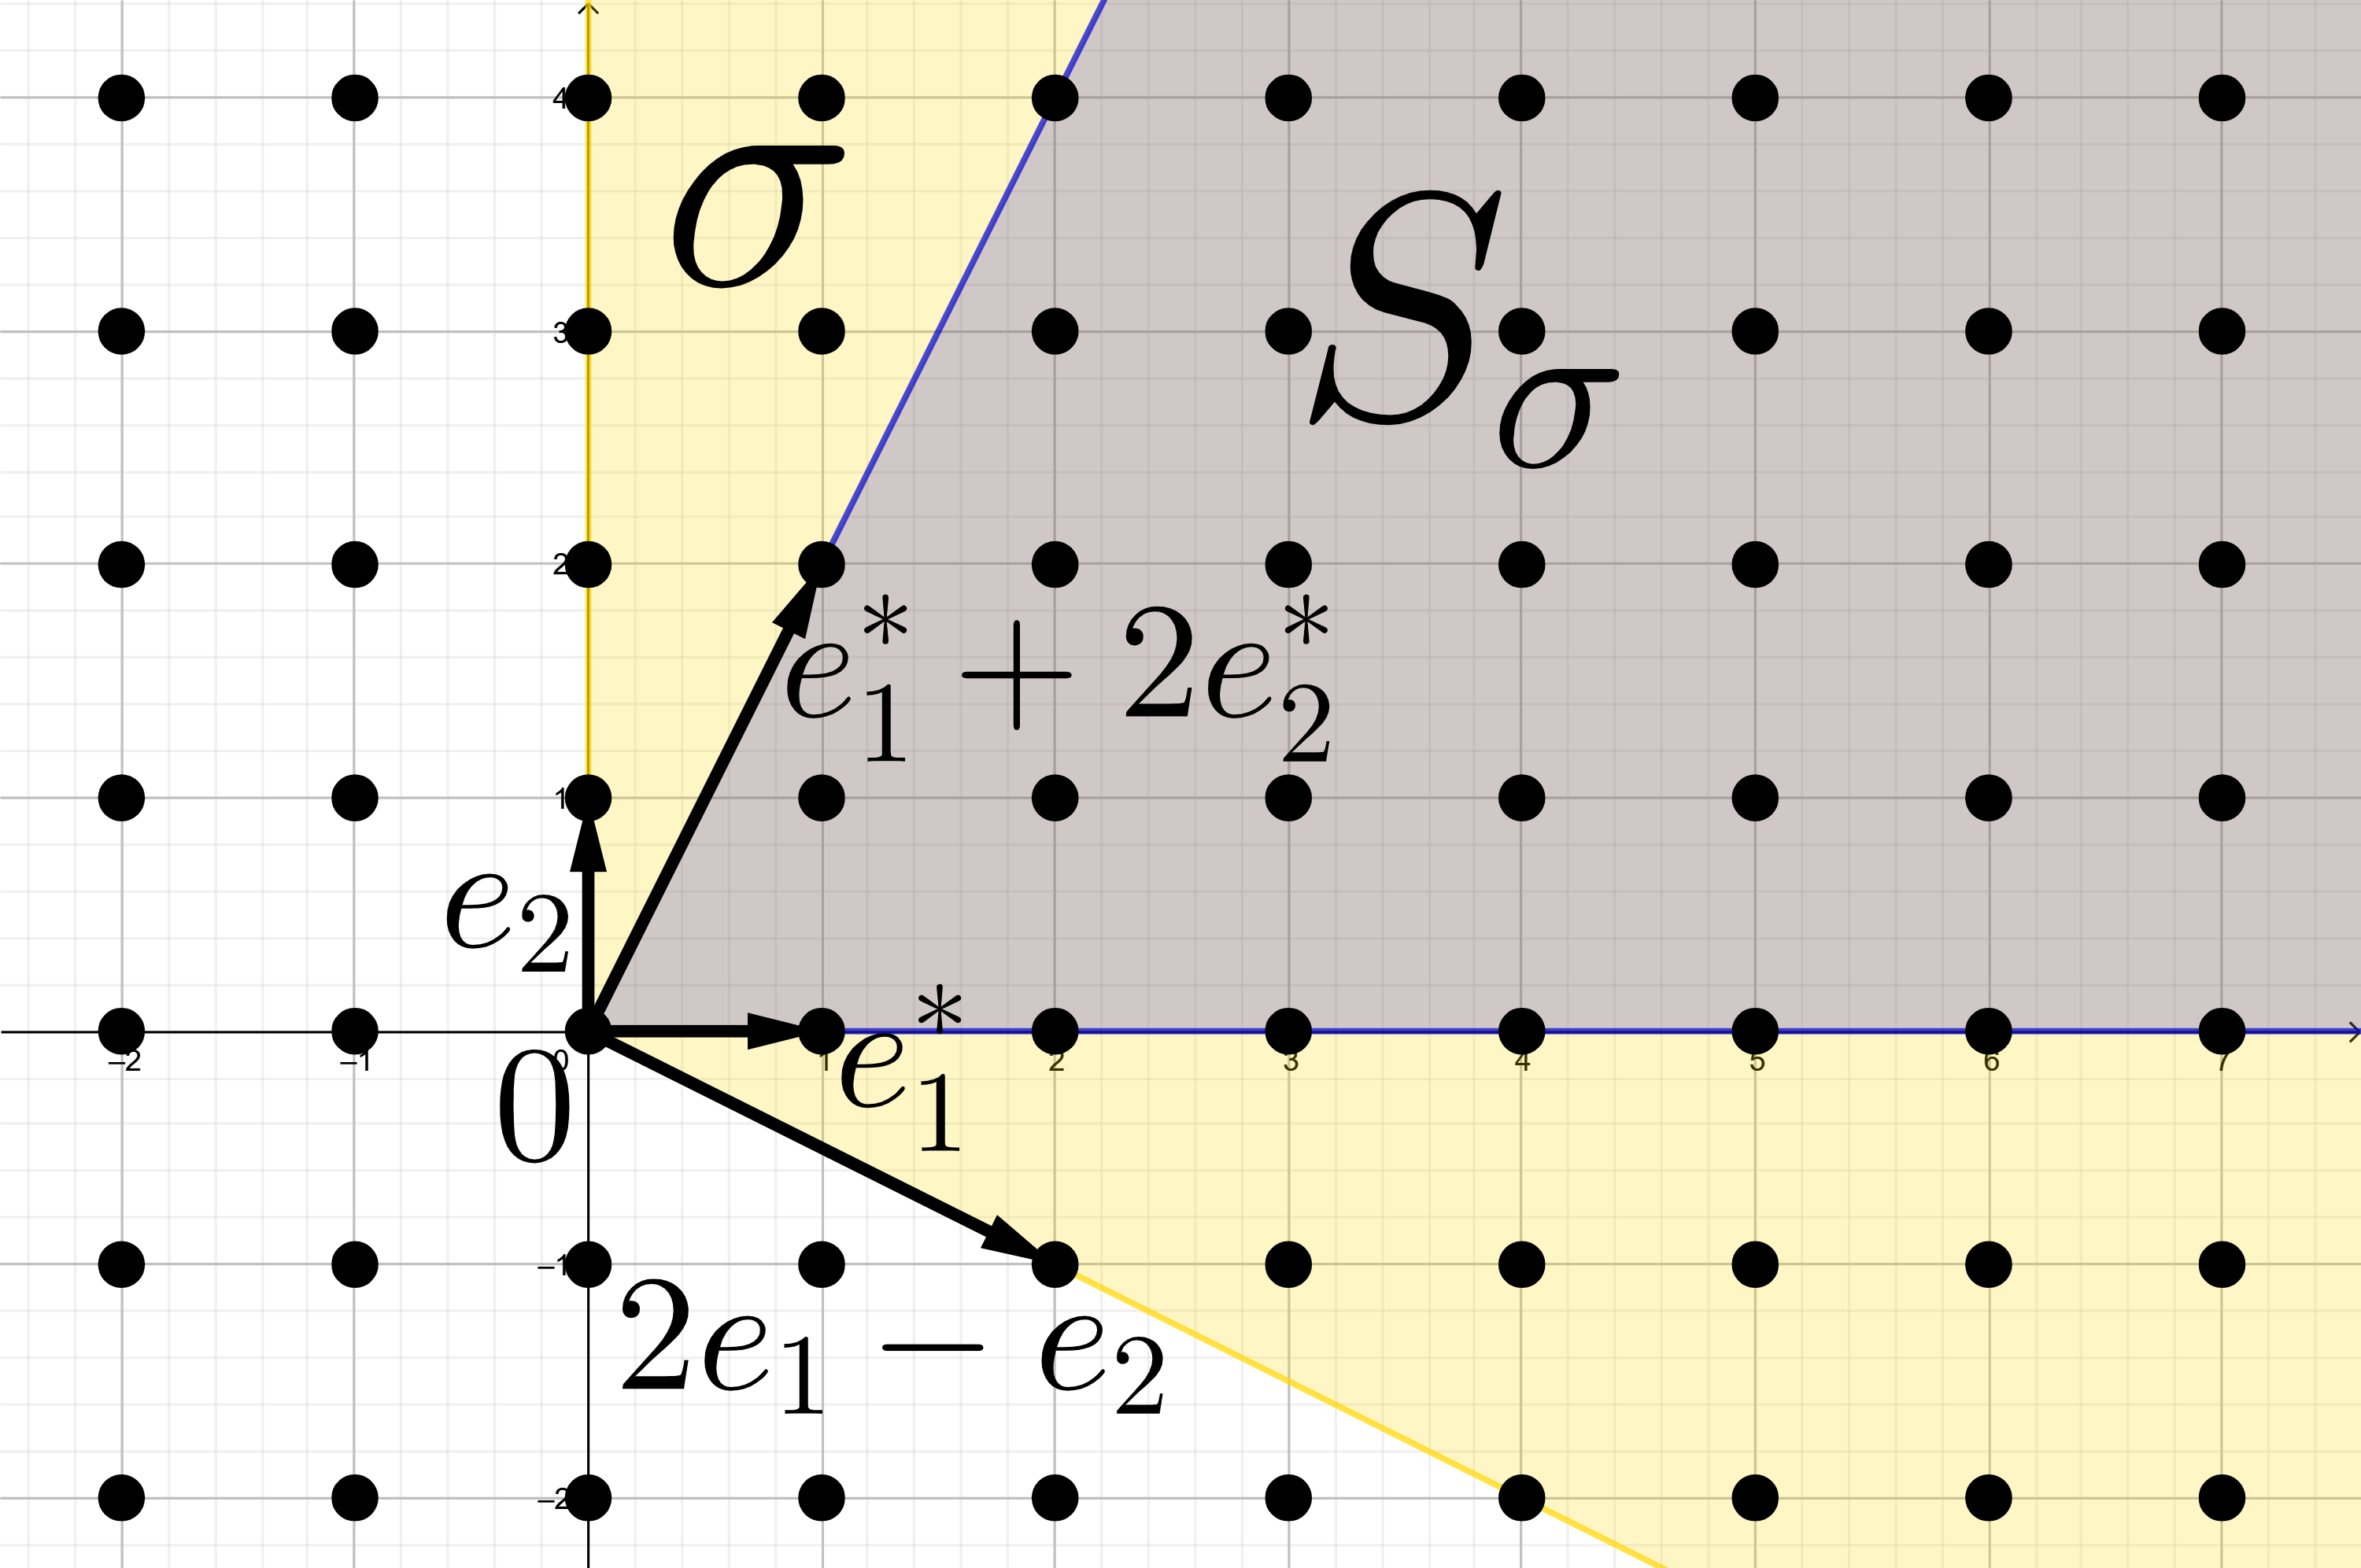
\includegraphics[scale=0.6]{Pictures/Cone.png}
\end{subfigure}
\begin{subfigure}{.35\textwidth}
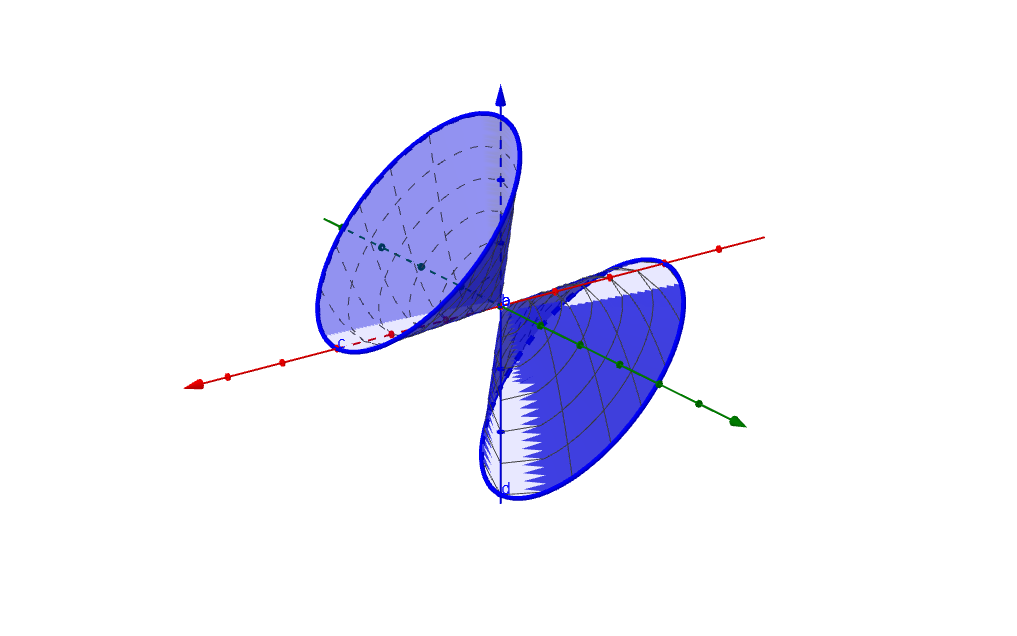
\includegraphics[scale=0.29]{Pictures/Variety.png}
\end{subfigure}
\end{center}
\end{figure}
%
%\item Let $\sigma\subseteq\mathbb{R}^3$ be the cone generated by $e_1,e_2,e_3,e_1+e_3-e_2$. Let's calculate the generators of $S_{\sigma}$.
%
%The cone $\sigma$ has dimension 3, so its facets have dimension 2. Recall that the facets are generated by subsets of the generators of $\sigma$. There are six possibilities:
%\[\tau_1:\{e_2,e_3\},\tau_2:\{e_1,e_2\},\tau_3:\{e_3,e_1+e_3-e_2\},\tau_4:\{e_1,e_1+e_3-e_2\},\]\[\tau_5:\{e_1,e_3\},\tau_6:\{e_2,e_1+e_3-e_2\}.\]
%Let $u_i\in(\mathbb{R}^3)^*$ such that $\tau_i=\sigma\cap u_i^{\perp}$.
%\[u_1=e_1^*\in\sigma^{\vee},u_2=e_3^*\in\sigma^{\vee},u_3=e_1^*+e_2^*\in\sigma^{\vee},u_4=e_2^*+e_3^*\in\sigma^{\vee},u_5=\pm e_2\notin\sigma^{\vee},\pm(e_1^*-e_3^*)\notin\sigma^{\vee}.\]
%
%The generators of $S_{\sigma}$ are
%\[\{t_1u_1+t_2u_2+t_3u_3+t_4u_4\,|\,0\leq t_1,t_2,t_3,t_4\leq1\}.\]
%
%Then $S_{\sigma}$ is generated by $e_1^*,e_3^*,e_1^*+e_2^*,e_2^*+e_3^*$. Hence,
%\[A_{\sigma}=\mathbb{C}[X_1,X_3,X_1X_2,X_2X_3]=\mathbb{C}[W,X,Y,Z]/(WZ-XY),\]
%\[U_{\sigma}=\Spec\mathbb{C}[W,X,Y,Z]/(WZ-XY)=V(WZ-XY)=\{(W,X,Y,Z)\in\mathbb{C}^4\,|\,WZ=XY\}.\]
%
%The affine toric variety of this cone is the hypersurface $WZ=XY$ in $\mathbb{C}^4$.
\end{enumerate}
\end{example}
\end{document}
